
\setcounter{chapter}{1}
\chapter{Project Development Practices}
\minitoc %insert la minitoc
\graphicspath{{Chapter2/figures/}}

%\DoPToC

%==============================================================================
\pagestyle{fancy}
\fancyhf{}
\fancyhead[R]{\bfseries\rightmark}
\fancyfoot[R]{\thepage}
\renewcommand{\headrulewidth}{0.5pt}
\renewcommand{\footrulewidth}{0pt}
\renewcommand{\chaptermark}[1]{\markboth{\MakeUppercase{\chaptername~\thechapter. #1 }}{}}
\renewcommand{\sectionmark}[1]{\markright{\thechapter.\thesection~ #1}}

\begin{spacing}{1.2}
%==============================================================================
\section*{Introduction}
In this chapter we will set the basis for the development of our project. we will define a set of development practices to follow and the list of tools to use in the making of the final product.
\section{Mock-ups}
To guarantee a good control of our project and to simplify the interaction with the final users, we support our analysis of functional needs with mock-ups that model the different interfaces of our final product. These models are made by the "Adobe XD" tool.
\subsection{Mock-ups Examples}
\begin{figure}[!h]\centering
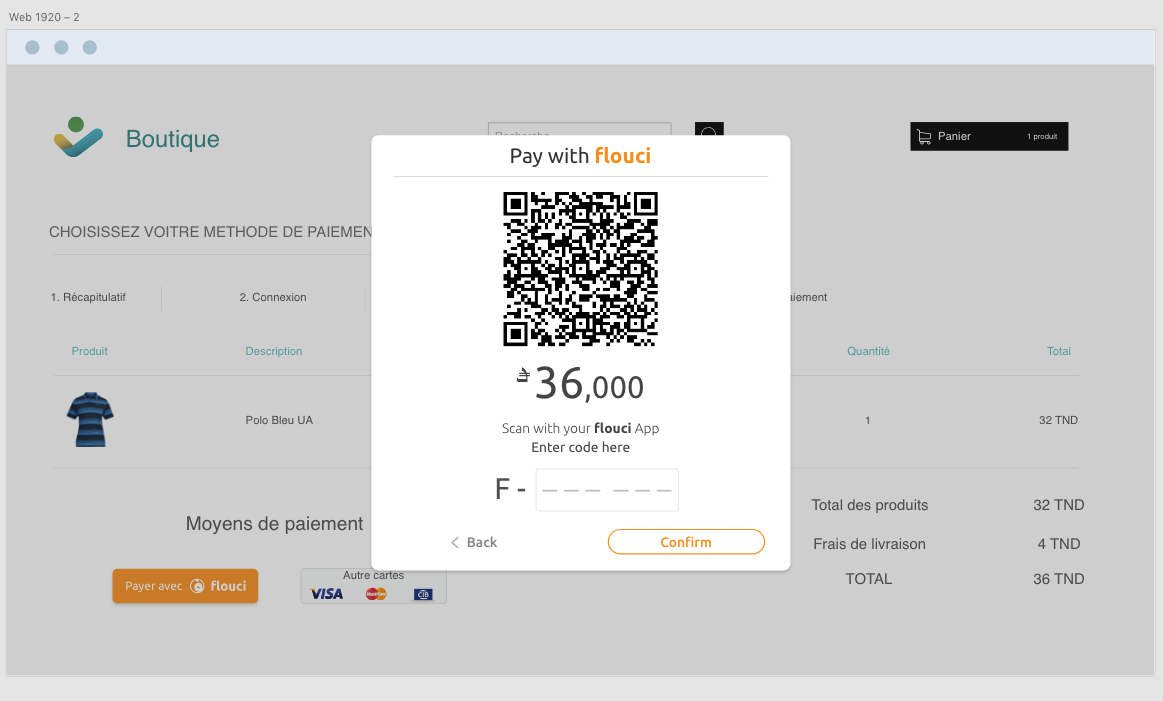
\includegraphics[scale=0.4]{Checkout_screen}
\caption{Checkout Mock-Up}
\label{fig:fig1}
\end{figure}

\begin{figure}[!h]\centering
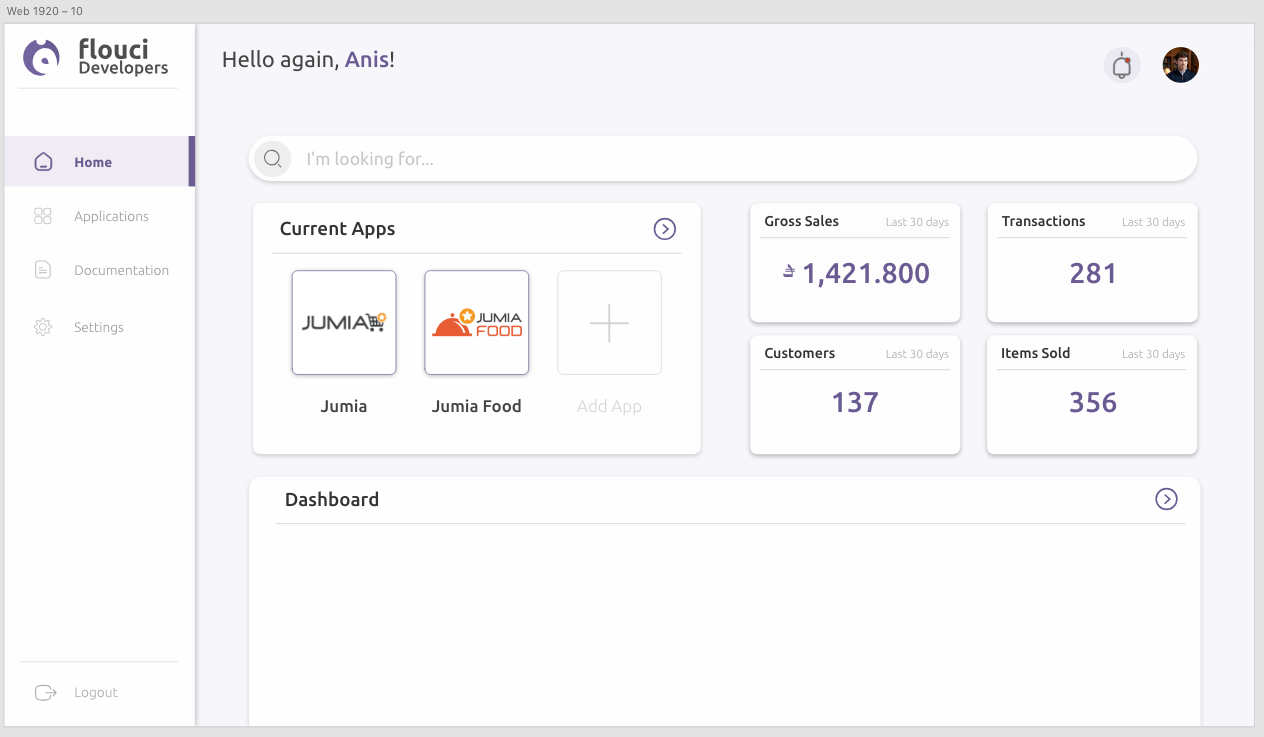
\includegraphics[scale=0.4]{web_screen}
\caption{Checkout Mock-Up}
\label{fig:fig1}
\end{figure}

\section*{Conclusion}

%==============================================================================
\end{spacing}
